

%% NJCTL: PSI AP Physics C
%%----------------------------------------


%% Work and Energy with Algebra
%%----------------------------------------
\element{njctl}{
\begin{question}{work-algebra-Q01}
    A student throws a ball upwards from the ground level where gravitational potential energy is zero.
    At a height of \SI{15}{\meter},
        the ball has a potential energy of \SI{60}{\joule},
        and is moving upwards with a kinetic energy of \SI{40}{\joule}.
    Ignoring air resistance,
        the maximum height achieved by the ball is most nearly:
    \begin{multicols}{3}
    \begin{choices}
        \wrongchoice{\SI{10}{\meter}}
        \wrongchoice{\SI{20}{\meter}}
      \correctchoice{\SI{25}{\meter}}
        \wrongchoice{\SI{30}{\meter}}
        \wrongchoice{\SI{40}{\meter}}
    \end{choices}
    \end{multicols}
\end{question}
}

\element{njctl}{
\begin{question}{work-algebra-Q02}
    A box of mass $m$ is lifted a vertical distance $h$ in time $t$ with a constant velocity.
    The power supplied by the lifting force is approximately:
    \begin{multicols}{3}
    \begin{choices}
        \wrongchoice{$mght$}
      \correctchoice{$\dfrac{mgh}{t}$}
        \wrongchoice{zero}
        \wrongchoice{$\dfrac{mgt}{h}$}
        \wrongchoice{$\dfrac{mg}{h5}$}
    \end{choices}
    \end{multicols}
\end{question}
}

\element{njctl}{
\begin{question}{work-algebra-Q03}
    A crate is lifted by a force $F$ which is greater in magnitude than the crate's weight $W$.
    The change in kinetic energy of the crate during this time is equal to the
    \begin{choices}
      \correctchoice{work done by the net force $(F-W)$.}
        \wrongchoice{work done by $F$.}
        \wrongchoice{work done by $W$.}
        \wrongchoice{the change in momentum of the rock before and after this time.}
        \wrongchoice{the change in the potential energy of the rock before and after this time.}
    \end{choices}
\end{question}
}

\element{njctl}{
\begin{question}{work-algebra-Q04}
    A constant force supplies an average power of \SI{8}{\watt} to a box during a certain time interval.
    If the box has an average speed of \SI{4}{\meter\per\second} and the force acts in the same direction as motion of the object,
        the magnitude of the force is
    \begin{multicols}{3}
    \begin{choices}
        \wrongchoice{\SI{8}{\newton}}
        \wrongchoice{\SI{6}{\newton}}
        \wrongchoice{\SI{4}{\newton}}
      \correctchoice{\SI{2}{\newton}}
        \wrongchoice{\SI{1}{\newton}}
    \end{choices}
    \end{multicols}
\end{question}
}

\element{njctl}{
\begin{question}{work-algebra-Q05}
    A pencil is moved from point $A$ to point $B$ along a curved path.
    \begin{center}
    \begin{tikzpicture}
        %% NOTE:
    \end{tikzpicture}
    \end{center}
    The work done by the gravitational force on the pencil depends on which of the following:
    \begin{choices}
        \wrongchoice{the velocity of the object as it moves between $A$ and $B$}
      \correctchoice{the positions of points $A$ and $B$}
        \wrongchoice{the path taken between $A$ and $B$}
        \wrongchoice{both the positions of $A$ and $B$ and the path taken between them}
        \wrongchoice{the nature of the external force that moves the object from $A$ to $B$}
    \end{choices}
\end{question}
}

\element{njctl}{
\begin{question}{work-algebra-Q06}
    A student lifts a mass $m$ at constant speed to a height $h$ in time $t$.
    How much work is done by the student?
    \begin{multicols}{3}
    \begin{choices}
        \wrongchoice{$mgt$}
        \wrongchoice{zero}
      \correctchoice{$mgh$}
        \wrongchoice{$\dfrac{mgh}{t}$}
        \wrongchoice{$\dfrac{mgt}{h}$}
    \end{choices}
    \end{multicols}
\end{question}
}

\element{njctl}{
\begin{question}{work-algebra-Q07}
    A \SI{3}{\meter} long frictionless pendulum swings with a maximum angular displacement of \ang{10} from the vertical.
    At its lowest position,
        the kinetic energy of the pendulum is \SI{20}{\joule}.
    What is the potential energy of the pendulum when the kinetic energy is \SI{5}{\joule}?
    \begin{multicols}{3}
    \begin{choices}
        \wrongchoice{\SI{3.3}{\joule}}
        \wrongchoice{\SI{5}{\joule}}
        \wrongchoice{\SI{6.7}{\joule}}
        \wrongchoice{\SI{10}{\joule}}
      \correctchoice{\SI{15}{\joule}}
    \end{choices}
    \end{multicols}
\end{question}
}

\element{njctl}{
\begin{question}{work-algebra-Q08}
    On top of a \SI{300}{\meter} skyscraper,
        a \SI{2}{\kilo\gram} ball is thrown directly downwards with an initial speed of \SI{20}{\meter\per\second}.
    If the ball reaches the ground with a speed of \SI{60}{\meter\per\second},
        the energy lost to friction is approximately:
    \begin{multicols}{3}
    \begin{choices}
        \wrongchoice{zero}
        \wrongchoice{\SI{1800}{\joule}}
        \wrongchoice{\SI{2300}{\joule}}
      \correctchoice{\SI{2800}{\joule}}
        \wrongchoice{\SI{3300}{\joule}}
    \end{choices}
    \end{multicols}
\end{question}
}

\element{njctl}{
\begin{question}{work-algebra-Q09}
    A student pushes a box across a rough,
        flat surface at a constant speed of \SI{1}{\meter\per\second}.
    The box has a mass of 50 kilograms,
        and the coefficient of sliding friction is \num{0.2}.
    The power supplied by the student to the box is:
    \begin{multicols}{3}
    \begin{choices}
        \wrongchoice{zero}
        \wrongchoice{\SI{5}{\watt}}
        \wrongchoice{\SI{50}{\watt}}
      \correctchoice{\SI{100}{\watt}}
        \wrongchoice{\SI{200}{\watt}}
    \end{choices}
    \end{multicols}
\end{question}
}

\element{njctl}{
\begin{question}{work-algebra-Q10}
    A ball of mass $m$ is suspended at the end of a massless string of length $L$ as shown below.
    \begin{center}
    \begin{tikzpicture}
        %% Ceiling
        \node[anchor=south,fill,pattern=north east lines,minimum width=4cm, minimum height=0.05cm] at (0,0) {};
        \draw (-2,0) -- (2,0);
        %% Mass
        \draw[dashed] (270:3) arc (270:325:3);
        \node[draw,circle,fill=white!90!black,minimum size=1em,anchor=center] (A) at (270:3) {$m$};
        \node[draw,dashed,fill=white,circle,minimum size=1em,anchor=center] (B) at (325:3) {$m$};
        %% String
        \draw (0,0) -- (A.north);
        \draw (0,0) -- (B.north west);
        %% Angle
        \draw[<->] (270:1) arc(270:324:1) node[pos=0.5,anchor=north] {\ang{45}};
        %% Length
        \draw[thick,<->] (-1,0) -- (-1,-3) node[pos=0.5,anchor=center,fill=white] {$L$};
    \end{tikzpicture}
    \end{center}
    This pendulum is lifted to a \ang{45} angle with the vertical and released.
    At the low point of its swing,
        the speed of the ball is:
    \begin{multicols}{2}
    \begin{choices}
        \wrongchoice{$\sqrt{gL}$}
        \wrongchoice{$\sqrt{2gL}$}
      \correctchoice{$\sqrt{gL\left(2-\sqrt{2}\right)}$}
        \wrongchoice{$gL$}
        \wrongchoice{$\dfrac{1}{2gL}$}
    \end{choices}
    \end{multicols}
\end{question}
}

\element{njctl}{
\begin{question}{work-algebra-Q11}
    A \SI{5}{\kilo\gram} block is pushed horizontally,
        at a constant speed of \SI{3}{\meter\per\second},
        across a rough surface with a coefficient of kinetic friction of \num{0.2} by a force $F$.
    The work that is done by force $F$ in \SI{20}{\second} is:
    \begin{multicols}{3}
    \begin{choices}
        \wrongchoice{\SI{200}{\joule}}
        \wrongchoice{\SI{400}{\joule}}
      \correctchoice{\SI{600}{\joule}}
        \wrongchoice{\SI{800}{\joule}}
        \wrongchoice{\SI{1000}{\joule}}
    \end{choices}
    \end{multicols}
\end{question}
}

\element{njctl}{
\begin{question}{work-algebra-Q12}
    A spring gun with a spring constant $k$ launches a ball of mass m off a cliff of height $h$.
    If the velocity of the ball right before it hits the ground is $v$,
        how much was the spring compressed?
    \begin{multicols}{2}
    \begin{choices}
        \wrongchoice{zero}
        \wrongchoice{$mgh$}
        \wrongchoice{$\dfrac{1}{2}mv$}
        \wrongchoice{$\sqrt{\dfrac{wmgh}{k}}$}
      \correctchoice{$\sqrt{\dfrac{m\left(v^2-2gh\right)}{k}}$}
    \end{choices}
    \end{multicols}
\end{question}
}

\element{njctl}{
\begin{question}{work-algebra-Q13}
    A \SI{10}{\kilo\gram} block is lifted \SI{5}{\meter} upward at a constant speed of \SI{2}{\meter\per\second}.
    What is the average power supplied?
    \begin{multicols}{3}
    \begin{choices}
      \correctchoice{\SI{200}{\watt}}
        \wrongchoice{\SI{120}{\watt}}
        \wrongchoice{\SI{20}{\watt}}
        \wrongchoice{\SI{25}{\watt}}
        \wrongchoice{\SI{50}{\watt}}
    \end{choices}
    \end{multicols}
\end{question}
}

\element{njctl}{
\begin{question}{work-algebra-Q14}
    A \SI{2}{\kilo\gram} mass accelerates for \SI{10}{\meter} across a frictionless surface by a \SI{40}{\newton} force as shown in the figure below.
    \begin{center}
    \begin{tikzpicture}
        %% Floor
        \node[anchor=north,fill,pattern=north east lines,minimum width=6cm, minimum height=0.05cm] at (0,0) {};
        \draw (-3,0) -- (3,0);
        %% Mass
        \node[draw,fill=white!90!black,minimum size=1.5cm,anchor=south] (A) at (-1,0) {\SI{2}{\kilo\gram}};
        %% Vectors
        \draw[thick,->] (A.east) -- ++(60:2) node[pos=0.5,anchor=south east] {\SI{40}{\newton}};
        \draw[dashed] (A.east) -- ++(0:1.5);
        \draw[<->] (A.east) ++(0:1) arc(0:60:1) node[pos=0.5,anchor=west] {\ang{60}};
    \end{tikzpicture}
    \end{center}
    The work done over this interval is:
    \begin{multicols}{3}
    \begin{choices}
        \wrongchoice{$120\,\si{\joule}$}
        \wrongchoice{$200\sqrt{3}\,\si{\joule}$}
        \wrongchoice{$120\sqrt{3}\,\si{\joule}$}
        \wrongchoice{$400\,\si{\joule}$}
      \correctchoice{$200\,\si{\joule}$}
    \end{choices}
    \end{multicols}
\end{question}
}

\newcommand{\PSIapcWorkAlgebraQFifteen}{
\begin{tikzpicture}
    \begin{axis}[
        axis y line=left,
        axis x line=middle,
        axis line style={->},
        xlabel={position},
        x unit=\si{\meter},
        xtick={0,2,4,6},
        minor x tick num=1,
        ylabel={force},
        y unit=\si{\newton},
        ytick={-2,0,2,4},
        minor y tick num=1,
        xmin=0,xmax=6.5,
        ymin=-2.5,ymax=4.5,
        width=0.8\columnwidth,
        height=0.5\columnwidth,
        grid=major,
        very thin,
    ]
    \addplot[line width=1pt,mark=\empty] plot coordinates {(0,4) (6,-2) };
    \end{axis}
\end{tikzpicture}
}

\element{njctl}{
\begin{question}{work-algebra-Q15}
    The graph below represents the force exerted on a particle.
    \begin{center}
        \PSIapcWorkAlgebraQFifteen
    \end{center}
    What is the work done on the object from $x=0$ to $x=\SI{4}{\meter}$?
    \begin{multicols}{3}
    \begin{choices}
      \correctchoice{\SI{8}{\joule}}
        \wrongchoice{\SI{10}{\joule}}
        \wrongchoice{\SI{15}{\joule}}
        \wrongchoice{\SI{16}{\joule}}
        \wrongchoice{\SI{20}{\joule}}
    \end{choices}
    \end{multicols}
\end{question}
}

\element{njctl}{
\begin{question}{work-algebra-Q16}
    The graph below represents the force exerted on a particle.
    \begin{center}
        \PSIapcWorkAlgebraQFifteen
    \end{center}
    What is the work done on the object from $x=0$ to $x=\SI{6}{\meter}$?
    \begin{multicols}{3}
    \begin{choices}
        \wrongchoice{\SI{4}{\joule}}
      \correctchoice{\SI{6}{\joule}}
        \wrongchoice{\SI{10}{\joule}}
        \wrongchoice{\SI{12.5}{\joule}}
        \wrongchoice{\SI{25}{\joule}}
    \end{choices}
    \end{multicols}
\end{question}
}

\element{njctl}{
\begin{question}{work-algebra-Q17}
    Which of the following is an accurate statement?
    \begin{choices}
        \wrongchoice{Potential energy is always negative.}
        \wrongchoice{Total energy is always positive.}
        \wrongchoice{During simple harmonic motion, the kinetic energy is always equal to the potential energy.}
      \correctchoice{Kinetic energy is never negative.}
        \wrongchoice{None of the provided are true.}
    \end{choices}
\end{question}
}

\element{njctl}{
\begin{question}{work-algebra-Q18}
    A stone is dropped from the edge of a cliff.
    Which of the following graphs best represents the stone's kinetic energy as a function of time?
    \begin{multicols}{2}
    \begin{choices}
        \AMCboxDimensions{down=-2.5em}
        \wrongchoice{
            \begin{tikzpicture}
                \begin{axis}[
                    axis y line=left,
                    axis x line=bottom,
                    axis line style={->},
                    xlabel={time},
                    xtick=\empty,
                    ylabel={energy},
                    ytick=\empty,
                    xmin=0,xmax=11,
                    ymin=0,ymax=11,
                    width=0.95\columnwidth,
                ]
                \addplot[line width=1pt,domain=0:10]{x};
                \end{axis}
            \end{tikzpicture}
        }
        %% ANS is B
        \correctchoice{
            \begin{tikzpicture}
                \begin{axis}[
                    axis y line=left,
                    axis x line=bottom,
                    axis line style={->},
                    xlabel={time},
                    xtick=\empty,
                    ylabel={energy},
                    ytick=\empty,
                    xmin=0,xmax=11,
                    ymin=0,ymax=11,
                    width=0.95\columnwidth,
                ]
                \addplot[line width=1pt,domain=0:10]{0.1*x*x};
                \end{axis}
            \end{tikzpicture}
        }
        \wrongchoice{
            \begin{tikzpicture}
                \begin{axis}[
                    axis y line=left,
                    axis x line=bottom,
                    axis line style={->},
                    xlabel={time},
                    xtick=\empty,
                    ylabel={energy},
                    ytick=\empty,
                    xmin=0,xmax=11,
                    ymin=0,ymax=11,
                    width=0.95\columnwidth,
                ]
                \addplot[line width=1pt,domain=0:10]{3+0.07*x*x};
                \end{axis}
            \end{tikzpicture}
        }
        \wrongchoice{
            \begin{tikzpicture}
                \begin{axis}[
                    axis y line=left,
                    axis x line=bottom,
                    axis line style={->},
                    xlabel={time},
                    xtick=\empty,
                    ylabel={energy},
                    ytick=\empty,
                    xmin=0,xmax=11,
                    ymin=0,ymax=11,
                    width=0.95\columnwidth,
                ]
                \addplot[line width=1pt,domain=0:10]{3+7*x/10};
                \end{axis}
            \end{tikzpicture}
        }
        \wrongchoice{
            \begin{tikzpicture}
                \begin{axis}[
                    axis y line=left,
                    axis x line=bottom,
                    axis line style={->},
                    xlabel={time},
                    xtick=\empty,
                    ylabel={energy},
                    ytick=\empty,
                    xmin=0,xmax=11,
                    ymin=0,ymax=11,
                    width=0.95\columnwidth,
                ]
                \addplot[line width=1pt,domain=0:10]{4};
                \end{axis}
            \end{tikzpicture}
        }
    \end{choices}
    \end{multicols}
\end{question}
}

\element{njctl}{
\begin{question}{work-algebra-Q19}
    A \SI{4}{\kilo\gram} ball is attached to a \SI{1.5}{\meter} long string and whirled in a horizontal circle at a constant speed \SI{5}{\meter\per\second}.
    How much work is done on the ball during one period?
    \begin{multicols}{3}
    \begin{choices}
        \wrongchoice{\SI{9}{\joule}}
        \wrongchoice{\SI{4.5}{\joule}}
      \correctchoice{zero}
        \wrongchoice{\SI{2}{\joule}}
        \wrongchoice{\SI{8}{\joule}}
    \end{choices}
    \end{multicols}
\end{question}
}

\newcommand{\PSIapcWorkAlgebraQTwenty}{
\begin{tikzpicture}
    %% Ceiling
    \node[anchor=south,fill,pattern=north east lines,minimum width=4cm, minimum height=0.05cm] at (0,0) {};
    \draw (-2,0) -- (2,0);
    %% Path
    \draw[dashed] (210:3) arc (210:330:3)
        node[pos=0.0,anchor=south] {$1$}
        node[pos=0.5,anchor=north] {$2$}
        node[pos=1.0,anchor=south] {$3$};
    \draw (0,0) -- (235:3);
    %% Mass
    \node[draw,circle,fill=white!90!black,minimum size=1em,anchor=center] (A) at (235:3) {$m$};
    %% Length
    \draw[dashed] (270:3) -- ++(0:3cm);
    \draw[dashed] (330:3) -- ++(0:1.0);
    \draw[thick,<->] (330:3) ++(0:0.5) -- ++(270:1.5) node[pos=0.5,anchor=center,fill=white] {\SI{2}{\meter}};
\end{tikzpicture}
}

\element{njctl}{
\begin{question}{work-algebra-Q20}
    %% Questions 20-21
    A ball swings from point 1 to point 3.
    Assuming that point 3 is \SI{2}{\meter} above the lowest point 2.
    \begin{center}
        \PSIapcWorkAlgebraQTwenty
    \end{center}
    What happens to the kinetic energy of the ball when it moves from point 1 to point 2?
    \begin{choices}
      \correctchoice{increases}
        \wrongchoice{decreases}
        \wrongchoice{remains the same}
        \wrongchoice{zero}
        \wrongchoice{more information is required}
    \end{choices}
\end{question}
}

\element{njctl}{
\begin{question}{work-algebra-Q21}
    %% Questions 20-21
    A ball swings from point 1 to point 3.
    Assuming that point 3 is \SI{2}{\meter} above the lowest point 2.
    \begin{center}
        \PSIapcWorkAlgebraQTwenty
    \end{center}
    What is the velocity of the ball at the lowest point 2?
    \begin{multicols}{3}
    \begin{choices}
        \wrongchoice{\SI{2.2}{\meter\per\second}}
        \wrongchoice{\SI{3.5}{\meter\per\second}}
        \wrongchoice{\SI{4.7}{\meter\per\second}}
        \wrongchoice{\SI{5.1}{\meter\per\second}}
      \correctchoice{\SI{6.3}{\meter\per\second}}
    \end{choices}
    \end{multicols}
\end{question}
}

\element{njctl}{
\begin{question}{work-algebra-Q22}
    A block with a mass of $m$ slides at a constant velocity $v_0$ on a horizontal frictionless surface.
    The block collides with a spring and comes to rest when the spring is compressed to the maximum value.
    \begin{center}
    \begin{tikzpicture}
        %% Ground
        \node[anchor=north,fill,pattern=north east lines,minimum width=6cm, minimum height=0.05cm] at (-2,0) {};
        \draw (-5,0) -- (1,0);
        %% block
        \node[draw,fill=white!90!black,minimum size=2em,anchor=south] (A) at (-4,0) {$m$};
        %% velocity
        \draw[thick,->] (A.east) -- ++(0:1) node[pos=0.5,anchor=south] {$v_0$};
        %% Wall and Spring
        \draw[fill=white!50!black] (0,0) rectangle (1em,1cm);
        %\draw[fill=white!50!black] (-2cm,0) rectangle (-2.1cm,2em);
        \draw[thick,decoration={aspect=0.2,segment length=2.0mm,amplitude=3mm,coil},decorate] (0,1em) -- (-2,1em) node[pos=0.5,anchor=south,yshift=3mm] {$k$};
    \end{tikzpicture}
    \end{center}
    If the spring constant is $k$,
        what is the maximum compression in the spring?
    \begin{multicols}{3}
    \begin{choices}
      \correctchoice{$v_0\sqrt{\dfrac{m}{k}}$}
        \wrongchoice{$\dfrac{mv_0}{k}$}
        \wrongchoice{$\sqrt{\dfrac{mv_0}{k}}$}
        \wrongchoice{$v_0\sqrt{\dfrac{k}{m}}$}
        \wrongchoice{$\dfrac{mv_0^2}{k}$}
    \end{choices}
    \end{multicols}
\end{question}
}

\newcommand{\PSIapcWorkAlgebraQTwentyThree}{
\begin{tikzpicture}
    %% Ground
    \draw[thick] (-1,0) -- (5,0);
    \node[anchor=north,fill,pattern=north east lines,minimum width=6cm, minimum height=0.05cm] at (2,0) {};
    %% Path
    \draw[thick] (-1,3) -- (0,3) to[out=0,in=180] (2,0) to[out=0,in=180] (4,1.33) to [out=0,in=135] (5,0.25);
    %% Mass
    \draw[thick] node[draw,fill=white!90!black,minimum size=0.5cm,anchor=south] (M) at (0,3) {$m$};
    %% Labels
    \node[anchor=south east] at (-0.5,3) {$A$};
    \node[anchor=south] at (2,0) {$B$};
    \node[anchor=south] at (4,1.33) {$C$};
    \draw[<->] (0,0) -- (0,3) node[pos=0.5,fill=white,anchor=center] {\SI{45}{\meter}};
    \draw[<->] (4,0) -- (4,1.25) node[pos=0.5,fill=white,anchor=center] {\SI{25}{\meter}};
\end{tikzpicture}
}

\element{njctl}{
\begin{question}{work-algebra-Q23}
    %% Questions 23-24
    A \SI{500}{\kilo\gram} roller coaster car starts from rest at point $A$ and moves down the curved track.
    Ignore any energy loss due to friction.
    \begin{center}
        \PSIapcWorkAlgebraQTwentyThree
    \end{center}
    Find the speed of the car at the lowest point $B$.
    \begin{multicols}{3}
    \begin{choices}
        \wrongchoice{\SI{10}{\meter\per\second}}
        \wrongchoice{\SI{20}{\meter\per\second}}
      \correctchoice{\SI{30}{\meter\per\second}}
        \wrongchoice{\SI{40}{\meter\per\second}}
        \wrongchoice{\SI{50}{\meter\per\second}}
    \end{choices}
    \end{multicols}
\end{question}
}

\element{njctl}{
\begin{question}{work-algebra-Q24}
    %% Questions 23-24
    A \SI{500}{\kilo\gram} roller coaster car starts from rest at point $A$ and moves down the curved track.
    Ignore any energy loss due to friction.
    \begin{center}
        \PSIapcWorkAlgebraQTwentyThree
    \end{center}
    Find the speed of the car when it reaches point C.
    \begin{multicols}{3}
    \begin{choices}
        \wrongchoice{\SI{10}{\meter\per\second}}
      \correctchoice{\SI{20}{\meter\per\second}}
        \wrongchoice{\SI{30}{\meter\per\second}}
        \wrongchoice{\SI{40}{\meter\per\second}}
        \wrongchoice{\SI{50}{\meter\per\second}}
    \end{choices}
    \end{multicols}
\end{question}
}

\element{njctl}{
\begin{question}{work-algebra-Q25}
    Two projectiles $A$ and $B$ are launched from the ground with velocities of \SI{50}{\meter\per\second} at \ang{60} and \SI{50}{\meter\per\second} at \ang{30} with respect to the horizontal.
    Assuming there is no air resistance involved,
        which projectile has greater kinetic energy when it reaches the highest point of its trajectory?
    \begin{choices}
        \wrongchoice{projectile $A$}
      \correctchoice{projectile $B$}
        \wrongchoice{They both have the same none zero kinetic energy.}
        \wrongchoice{They both have zero kinetic energy at the highest point.}
        \wrongchoice{More information is required.}
    \end{choices}
\end{question}
}

\newcommand{\PSIapcWorkAlgebraQTwentySix}{
\begin{tikzpicture}
    \begin{axis}[
        axis y line=left,
        axis x line=bottom,
        axis line style={->},
        xlabel={position},
        x unit=\si{\meter},
        xtick={0,2,4,6},
        minor x tick num=1,
        ylabel={force},
        y unit=\si{\newton},
        ytick={0,20,40,60},
        minor y tick num=1,
        xmin=0,xmax=6.5,
        ymin=0,ymax=65,
        width=0.8\columnwidth,
        height=0.5\columnwidth,
        grid=both,
    ]
    \addplot[line width=1pt,mark=\empty] plot coordinates {(0,0) (3,50) (6,0) };
    \end{axis}
\end{tikzpicture}
}

\element{njctl}{
\begin{question}{work-algebra-Q26}
    %% Questions 26-27
    An object with a mass of \SI{2}{\kilo\gram} is initially at rest at a position $x=0$.
    A non-constant force $F$ is applied to the object over \SI{6}{\meter}.
    \begin{center}
        \PSIapcWorkAlgebraQTwentySix
    \end{center}
    What is the total work done by $F$ on the object at the end of \SI{6}{\meter}?
    \begin{multicols}{3}
    \begin{choices}
        \wrongchoice{\SI{200}{\joule}}
      \correctchoice{\SI{150}{\joule}}
        \wrongchoice{\SI{170}{\joule}}
        \wrongchoice{\SI{190}{\joule}}
        \wrongchoice{\SI{180}{\joule}}
    \end{choices}
    \end{multicols}
\end{question}
}

\element{njctl}{
\begin{question}{work-algebra-Q27}
    %% Questions 26-27
    An object with a mass of \SI{2}{\kilo\gram} is initially at rest at a position $x=0$.
    A non-constant force $F$ is applied to the object over \SI{6}{\meter}.
    \begin{center}
        \PSIapcWorkAlgebraQTwentySix
    \end{center}
    What is the velocity of the object at \SI{6}{\meter}?
    \begin{multicols}{3}
    \begin{choices}
        \wrongchoice{\SI{150}{\meter\per\second}}
        \wrongchoice{\SI{25}{\meter\per\second}}
        \wrongchoice{\SI{300}{\meter\per\second}}
      \correctchoice{\SI{12}{\meter\per\second}}
        \wrongchoice{\SI{35}{\meter\per\second}}
    \end{choices}
    \end{multicols}
\end{question}
}

\element{njctl}{
\begin{question}{work-algebra-Q28}
    An object has \SI{150}{\joule} of kinetic energy after increasing its speed from \SI{5}{\meter\per\second} t \SI{15}{\meter\per\second}.
    Which of the following choices best represents the mas of the object?
    \begin{multicols}{3}
    \begin{choices}
        \wrongchoice{\SI{0.5}{\kilo\gram}}
      \correctchoice{\SI{1.5}{\kilo\gram}}
        \wrongchoice{\SI{2.2}{\kilo\gram}}
        \wrongchoice{\SI{3.4}{\kilo\gram}}
        \wrongchoice{\SI{5.6}{\kilo\gram}}
    \end{choices}
    \end{multicols}
\end{question}
}

\newcommand{\njctlWorkAlgebraQTwentyNine}{
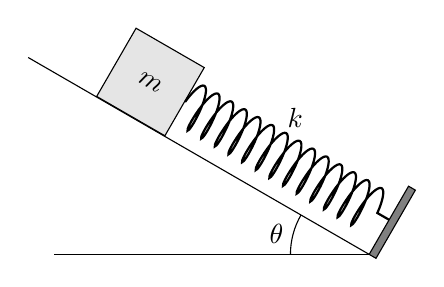
\begin{tikzpicture}
    %% Surface
    \draw (0,0) -- (150:5);
    \draw (0,0) -- (-4,0);
    \draw (-1,0) arc(180:150:1) node[pos=0.5,anchor=east] {$\theta$};
    %% block
    \node[draw,fill=white!90!black,minimum size=1cm,anchor=south,rotate=-30] (A) at (150:3.5) {$m$};
    %% Spring
    \draw[thick,decoration={aspect=0.2,segment length=2.0mm,amplitude=3mm,coil},decorate] (A.east) -- ++(330:3) node[pos=0.5,anchor=south,yshift=3mm,xshift=1mm] {$k$};
    %% Wall
    \draw[fill=white!50!black] (0,0) -- ++(60:1cm) -- ++(330:0.1) -- ++(240:1cm) -- cycle;
\end{tikzpicture}
}

\element{njctl}{
\begin{question}{work-algebra-Q29}
    A block of mass $m$ is at rest on the frictionless inclined plane with an incline angle of $\theta$.
    The block is just in a contact with the free end on an unstretched spring with a spring constant $k$.
    \begin{center}
        \njctlWorkAlgebraQTwentyNine
    \end{center}
    If the block is slowly moved down the incline
        (acceleration approximately equal to zero),
        what is the maximum compression in the spring?
    \begin{multicols}{3}
    \begin{choices}
        \wrongchoice{$kmg\sin\theta$}
        \wrongchoice{$kmg\cos\theta$}
      \correctchoice{$\dfrac{2mg\sin\theta}{k}$}
        \wrongchoice{$\dfrac{mg}{k}$}
        \wrongchoice{$kmg$}
    \end{choices}
    \end{multicols}
\end{question}
}

\element{njctl}{
\begin{question}{work-algebra-Q30}
    A box of mass $M$ begins at rest with point 1 at a height of $6R$,
        where $2R$ is the radius of the circular part of the track.
    The box slides down the frictionless track and around the loop.
    \begin{center}
    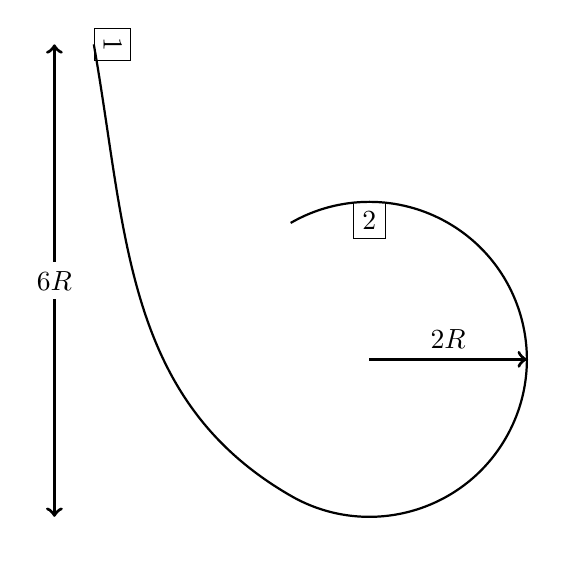
\begin{tikzpicture}
        %% Track
        \draw[thick] (-3.5,4) to[out=280,in=150] (240:2);
        \draw[thick] (240:2) arc(-120:120:2);
        \draw[very thick,->] (0,0) -- (2,0) node[pos=0.5,anchor=south] {$2R$};
        %% block 1
        \node[draw,minimum size=0.25,anchor=south,rotate=-90] at (-3.5,4) {$1$};
        %% block 2
        \node[draw,minimum size=0.25,anchor=north] at (90:2) {$2$};
        %% 6R
        \draw[very thick,<->] (-4,-2) -- (-4,4) node[pos=0.5,anchor=center,fill=white] {$6R$};
    \end{tikzpicture}
    \end{center}
    What is the ratio between the normal force on the box at point 2 to the box's weight?
    \begin{multicols}{3}
    \begin{choices}
      \correctchoice{$1:1$}
        \wrongchoice{$2:1$}
        \wrongchoice{$3:1$}
        \wrongchoice{$4:1$}
        \wrongchoice{$5:1$}
    \end{choices}
    \end{multicols}
\end{question}
}

\element{njctl}{
\begin{question}{work-algebra-Q31}
    A ball of mass $m$ is fastened to a string.
    The ball swings in a vertical circle of radius $r$ with the other end of the string held fixed.
    \begin{center}
    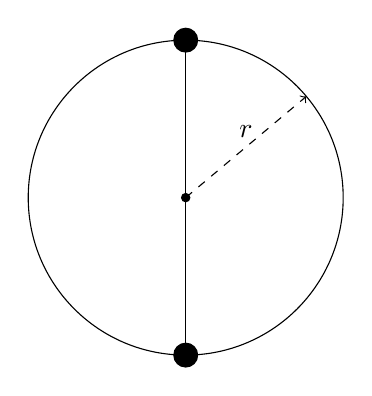
\begin{tikzpicture}
        %% path
        \draw (0,0) circle (2cm);
        \draw[fill] (0,0) circle (1.5pt);
        %% masses
        \draw (0,0) -- (90:2);
        \draw[fill] (90:2) circle (1ex);
        \draw (0,0) -- (270:2);
        \draw[fill] (270:2) circle (1ex);
        %% Radius
        \draw[dashed,->] (0,0) -- (40:2) node[pos=0.5,anchor=south] {$r$};
    \end{tikzpicture}
    \end{center}
    Neglecting air resistance,
        the difference between the string's tension at the bottom of the circle and at the top of the circle is:
    \begin{multicols}{3}
    \begin{choices}
        \wrongchoice{$mg$}
        \wrongchoice{$2mg$}
        \wrongchoice{$3mg$}
      \correctchoice{$6 mg$}
        \wrongchoice{$9 mg$}
    \end{choices}
    \end{multicols}
\end{question}
}

\element{njctl}{
\begin{question}{work-algebra-Q32}
    A system of two blocks is shown above.
    Block $A$ is placed on the surface of a rough horizontal table and on one side is connected to a vertical wall by an unstretched spring on the other is connected to block $B$ by a light string.
    The string passes over a frictionless and massless pulley.
    \begin{center}
    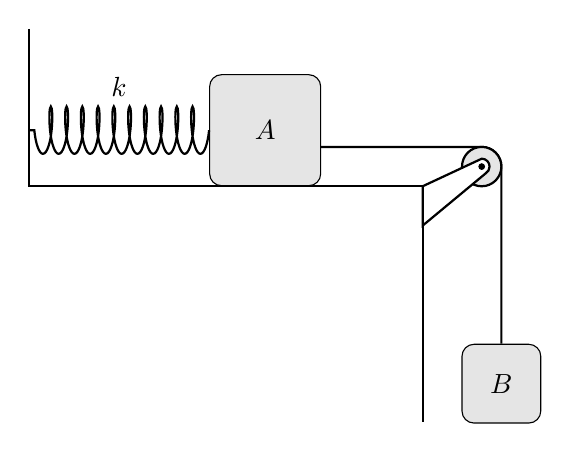
\begin{tikzpicture}
        %% Wall and Floor
        \draw[thick] (-3,2) -- (-3,0) -- (2,0) -- (2,-3);
        %% Mass
        \node[draw,fill=white!90!black,rectangle,rounded corners=1ex,minimum size=1.41cm,anchor=south] (A) at (0,0) {$A$};
        \node[draw,fill=white!90!black,rectangle,rounded corners=1ex,minimum size=1.00cm,anchor=north] (B) at (3,-2) {$B$};
        %% Rope
        \draw[thick] (A.south east) ++(90:0.5) -- (+2.75,0.5) arc(90:0:0.25) -- (B.north);
        %% Pully
        \draw[thick,fill=white!90!black] (+2.75,0.25) circle (0.25);
        \draw[thick,fill=white] (2,0) -- (2.75,0.35) arc (90:-60:0.1) -- (2,-0.5) -- cycle;
        \draw[fill] (+2.75,0.25) circle (1pt);
        %% spring
        \draw[thick,decoration={aspect=0.2,segment length=2.0mm,amplitude=3mm,coil},decorate] (A.west) -- ++(180:2.29) node[pos=0.5,anchor=south,yshift=3mm] {$k$};
    \end{tikzpicture}
    \end{center}
    Block $B$ is slowly moved down until it reaches the equilibrium position.
    Which of the following statements is true?
    \begin{choices}
        \wrongchoice{The total mechanical energy of the system is increased.}
        \wrongchoice{The loss in potential energy of block $B$ is equal to the work done by the friction force on block $A$.}
        \wrongchoice{The gain in potential energy of block $A$ is equal to the loss in potential energy of the spring.}
      \correctchoice{The gain in potential energy of block $A$ is greater than the loss in potential energy of the spring.}
        \wrongchoice{The gain in potential energy of block $A$ is less than the loss in potential energy of the spring.}
    \end{choices}
\end{question}
}

\element{njctl}{
\begin{question}{work-algebra-Q33}
    A crane can develop a \SI{2.5}{\kilo\watt} power output when lifting a metal block up.
    How long will it take for the crane to lift a \SI{250}{\kilo\gram} block at a constant speed to a height of \SI{5}{\meter} above the ground?
    \begin{multicols}{3}
    \begin{choices}
      \correctchoice{\SI{5}{\second}}
        \wrongchoice{\SI{10}{\second}}
        \wrongchoice{\SI{15}{\second}}
        \wrongchoice{\SI{20}{\second}}
        \wrongchoice{\SI{25}{\second}}
    \end{choices}
    \end{multicols}
\end{question}
}

\element{njctl}{
\begin{question}{work-algebra-Q34}
    A small block is released from rest at the top of a frictionless inclined plane.
    When the block reaches the bottom of the plane,
        it enters onto a rough horizontal surface.
    \begin{center}
    \begin{tikzpicture}
        %% NOTE:
        %% Ceiling
        \node[anchor=south,fill,pattern=north east lines,minimum width=4cm, minimum height=0.05cm] at (0,0) {};
    \end{tikzpicture}
    \end{center}
    How far does the block slide on the horizontal section before it comes to rest?
    \begin{multicols}{3}
    \begin{choices}
        %% NOTE: dimensional analysis
        \wrongchoice{$\dfrac{\mu g}{h}$}
        \wrongchoice{$\dfrac{\mu}{gh}$}
        \wrongchoice{$\dfrac{\mu}{h}$}
      \correctchoice{$\dfrac{h}{\mu}$}
        \wrongchoice{$\dfrac{h}{\mu g}$}
    \end{choices}
    \end{multicols}
\end{question}
}

\element{njctl}{
\begin{question}{work-algebra-Q35}
    Two blocks of masses \SI{0.5}{\kilo\gram} and \SI{0.75}{\kilo\gram} are connected with a light string that passes over a frictionless and massless pulley.
    \begin{center}
    \begin{tikzpicture}
        %% Ceiling
        \node[anchor=south,fill,pattern=north east lines,minimum width=3cm, minimum height=0.05cm] at (0,0) {};
        \draw (-1.5,0) -- (1.5,0);
        %% Masses
        \node[draw,fill=white!90!black,rectangle,rounded corners=1ex,minimum size=1.00cm] (A) at (-0.75,-4) {\SI{0.50}{\kilo\gram}};
        \node[draw,fill=white!90!black,rectangle,rounded corners=1ex,minimum size=1.22cm] (B) at (+0.75,-3) {\SI{0.75}{\kilo\gram}};
        %% Pulley
        \draw[thick] (0,-1.00) circle (0.75);
        \draw[fill=white!50!black] (-0.25,0) -- (-0.15,-1.1) arc(190:350:0.15) -- (0.25,0) --cycle;
        \draw[fill] (0,-1.00) circle (1.5pt);
        %% Rope
        \draw[thick] (A.north) -- (-0.75,-1) arc(180:0:0.75) -- (B.north);
    \end{tikzpicture}
    \end{center}
    What is the change in gravitational potential energy and change in kinetic energy of the system,
        \SI{2}{\second} after it released from rest?
    \begin{choices}
        \wrongchoice{$\Delta PE=\SI{+10}{\joule}$,  $\Delta KE=\SI{+10}{\joule}$}
        \wrongchoice{$\Delta PE=\SI{-10}{\joule}$,  $\Delta KE=\SI{-10}{\joule}$}
        \wrongchoice{$\Delta PE=\SI{+10}{\joule}$,  $\Delta KE=\SI{-10}{\joule}$}
      \correctchoice{$\Delta PE=\SI{-10}{\joule}$,  $\Delta KE=\SI{+10}{\joule}$}
        %% \text{zero} or 0 J ?
        \wrongchoice{$\Delta PE=\SI{0}{\joule}$,\phantom{+1}    $\Delta KE=\SI{0}{\joule}$}
    \end{choices}
\end{question}
}

\element{njctl}{
\begin{question}{work-algebra-Q36}
    A \SI{2500}{\kilo\gram} car accelerates from rest at a constant rate of \SI{2}{\meter\per\second\squared}.
    What power is required to increase the car's speed to \SI{20}{\meter\per\second}?
    \begin{multicols}{2}
    \begin{choices}
        %% Kilowatts?
        \wrongchoice{\SI{10 000}{\watt}}
        \wrongchoice{\SI{25 000}{\watt}}
        \wrongchoice{\SI{30 000}{\watt}}
        \wrongchoice{\SI{35 000}{\watt}}
      \correctchoice{\SI{50 000}{\watt}}
    \end{choices}
    \end{multicols}
\end{question}
}

\element{njctl}{
\begin{question}{work-algebra-Q37}
    A block of mass $m$ is placed on the frictionless inclined plane with an incline angle of $\theta$.
    The block is just in a contact with the free end on an unstretched spring with a spring constant $k$.
    \begin{center}
        \njctlWorkAlgebraQTwentyNine
    \end{center}
    If the block is released from rest,
        which of the following is true when it moves down the incline?
    \begin{multicols}{2}
    \begin{choices}
        %% NOTE: ANS is D
        \wrongchoice{}
        %Work done by gravity on block
        %Work done by spring on block
        %(A) Positive Positive
        %(B) Negative Negative
        %(C) Negative Positive
        %(D) Positive Negative
        %(E) Zero Zero
    \end{choices}
    \end{multicols}
\end{question}
}

\element{njctl}{
\begin{question}{work-algebra-Q38}
    A constant force $F=\SI{100}{\newton}$ pushes a \SI{5}{\kilo\gram} box \SI{10}{\meter} upward along the inclined plane.
    \begin{center}
    \begin{tikzpicture}
        %% NOTE:
    \end{tikzpicture}
    \end{center}
    Which of the following choices best represents the work done by the force $F$ on the box?
    \begin{multicols}{3}
    \begin{choices}
        \wrongchoice{\SI{250}{\joule}}
        \wrongchoice{\SI{866}{\joule}}
        \wrongchoice{\SI{500}{\joule}}
        \wrongchoice{\SI{765}{\joule}}
      \correctchoice{\SI{966}{\joule}}
    \end{choices}
    \end{multicols}
\end{question}
}

\element{njctl}{
\begin{question}{work-algebra-Q39}
    An external force is applied to a system of two blocks.
    \begin{center}
    \begin{tikzpicture}
        %% NOTE:
    \end{tikzpicture}
    \end{center}
    Which of the following is true if the blocks do not move with respect to each other?
    \begin{multicols}{2}
    \begin{choices}
        %% NOTE: ANS is D
        \wrongchoice{}
        %Work done by friction on block A
        %$Work done by friction on block B
        %(A) Positive Positive
        %(B) Negative Negative
        %(C) Positive Negative
        %(D) Negative Positive
        %(E) Zero Zero
    \end{choices}
    \end{multicols}
\end{question}
}

\element{njctl}{
\begin{question}{work-algebra-Q40}
    A car is traveling on a level road with an initial velocity $v_0$.
    If the coefficient of kinetic friction between the road and the tires is $\mu$,
        what is the shortest distance the car can travel after the driver locks the breaks?
    \begin{multicols}{3}
    \begin{choices}
      \correctchoice{$\dfrac{v_0^2}{2\mu g}$}
        \wrongchoice{$\dfrac{v_0^2}{\mu g}$}
        \wrongchoice{$\dfrac{v_0^2}{2\mu}$}
        \wrongchoice{$\dfrac{v_0}{2\mu g}$}
        \wrongchoice{$\dfrac{v_0^2}{2g}$}
    \end{choices}
    \end{multicols}
\end{question}
}


\endinput


